\section{Results}
\label{sec:results}


\subsection{Benchmarks and comparison with existing casters}

window size of $1024 \times 768$ pixels

\subsubsection{Cylinder head}

\begin{tabular}{r r r r r r r}
Volumes & Unique triangles & Cell triangles & Grid dimensions & Outside & Surface & Inside \\
\hline
21 & 28000 & 63604 & 40 40 18 & 13392 & 8744 & 6664 \\
\end{tabular}

update time 130
transfer 4

% 26 27 25 24 25 25 25 26 27 27
SingleBooleanCellRayCaster single 25.7 ms
% 72 72 74 72 72 72 72 72 75 72
SingleBooleanCellRayCaster double 72.5 ms
% 26 26 25 26 25 25 26 26 25 26
SinglePrimaryBooleanCellRayCaster single 25.6 ms
% 83 82 83 82 85 82 82 82 82 82
SinglePrimaryBooleanCellRayCaster double 82.5 ms
% 52 71 62 69 70 64 70 73 78 70
PacketRayCaster single 67.9 ms
% 47 41 42 48 39 46 46 46 46 48
CPU 44.9 ms

\subsubsection{Menger sponge 5}

\begin{tabular}{r r r r r r r}
Volumes & Unique triangles & Cell triangles & Grid dimensions & Outside & Surface & Inside \\
\hline
14044 & 168528 & 9582636 & 100 100 100 & 498480 & 501520 & 0 \\
\end{tabular}

update time 11071
transfer 177

% 42 42 42 41 41 41 42 42 41 42
SinglePrimaryBooleanCellRayCaster single 41.6 ms
% 260 258 259 259 259 258 258 258 258 258
SinglePrimaryBooleanCellRayCaster double 258.5 ms
% 41 40 43 43 40 40 40 40 40 40
SingleBooleanCellRayCaster single 40.7 ms
% 160 161 161 160 159 159 160 160 159 160
SingleBooleanCellRayCaster double 159.9 ms
% 880 479 679 675 336 447 641 425 1144 1448
PacketRayCaster single 715.4 ms
% 183 161 163 162 181 162 173 151 160 162
CPU 165.8 ms

\begin{figure}
\centering
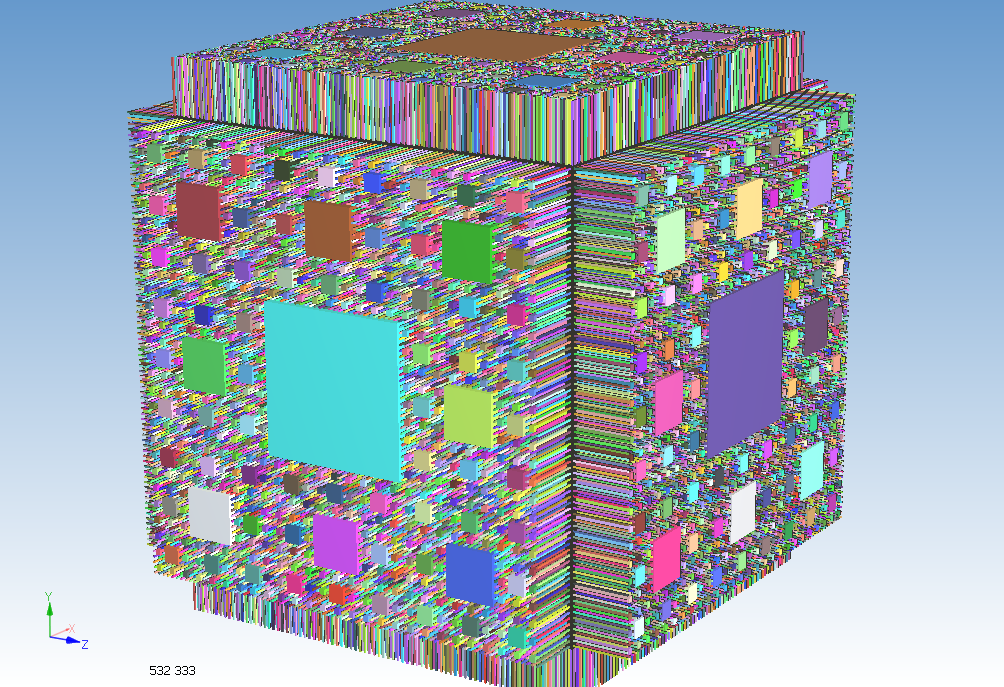
\includegraphics[width=0.49\textwidth]{menger_sponge_gl}
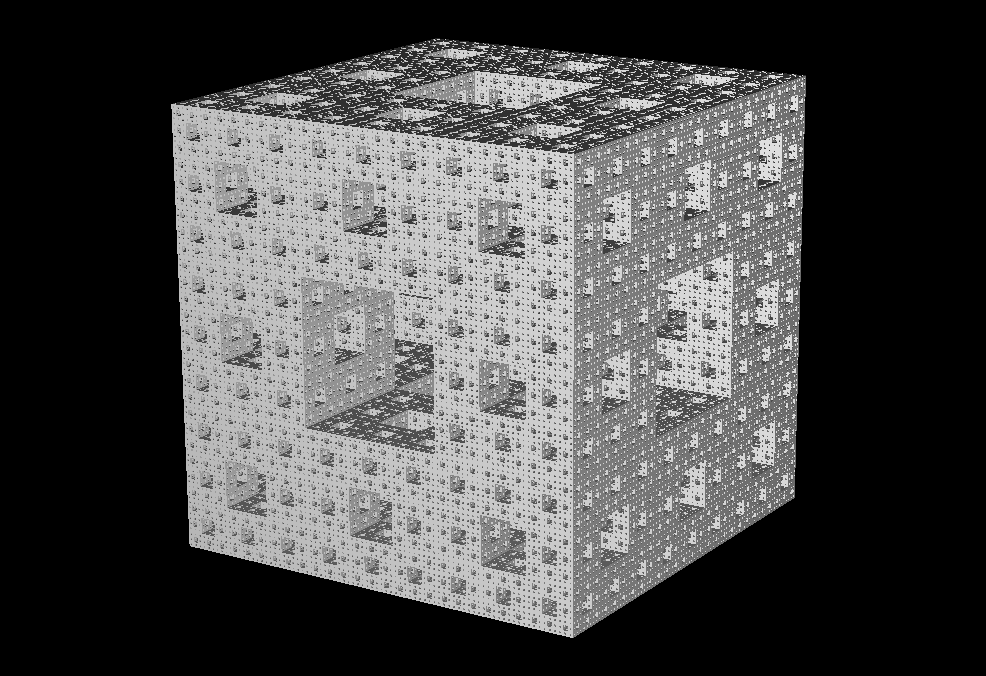
\includegraphics[width=0.49\textwidth]{menger_sponge}
\caption{Screenshot of the OpenCL kernel output of the SinglePrimaryBooleanCellRayCaster of a level 5 menger sponge.}
\label{fig:menger_sponge}
\end{figure}

\subsubsection{Multi impeller}

\begin{tabular}{r r r r r r r}
Volumes & Unique triangles & Cell triangles & Grid dimensions & Outside & Surface & Inside \\
\hline
4726 & 12510260 & 4010800 & 150 150 150 & 928405 & 139271 & 304824 \\
\end{tabular}

update time 10455
transfer 1086

% 124 123 123 123 123 123 123 123 124 123
SinglePrimaryBooleanCellRayCaster single 123.2 ms
% 959 954 961 958 953 954 951 959 956 952
SinglePrimaryBooleanCellRayCaster double 955.7 ms
% 114 114 114 114 113 113 115 114 114 115
SingleBooleanCellRayCaster single 114 ms
% 655 654 653 654 653 654 655 654 652 653
SingleBooleanCellRayCaster double 653.7 ms
% 1212 925 695 817 738 680 1512 824 714 1024
PacketRayCaster single 914.1 ms
% 324 321 314 326 313 313 313 322 314 300
CPU 316 ms

\begin{figure}
\centering
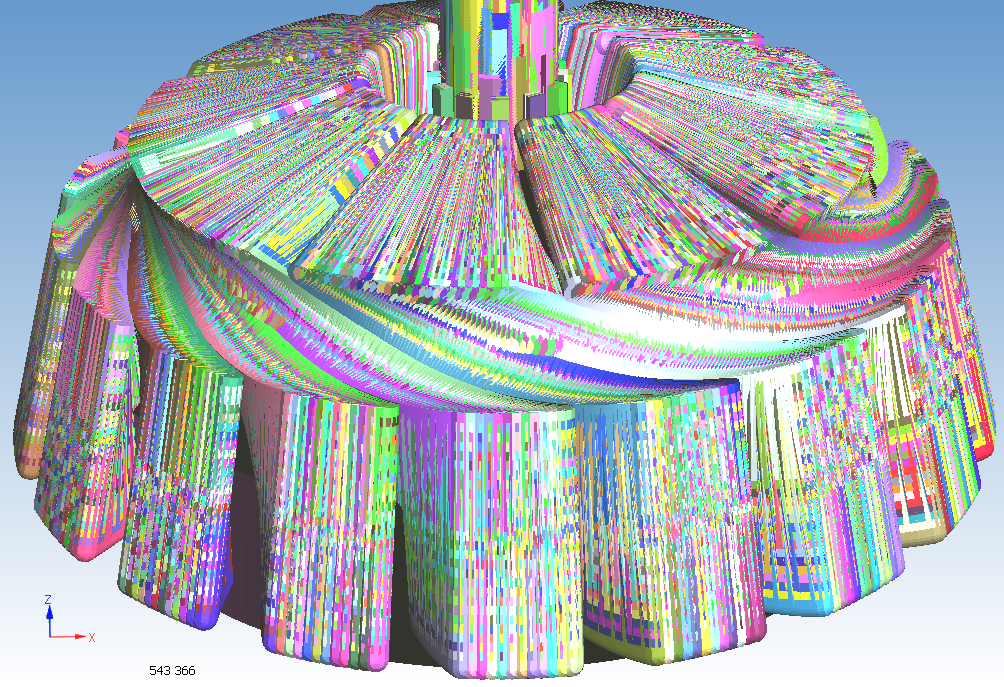
\includegraphics[width=0.49\textwidth]{multi_impeller_gl}
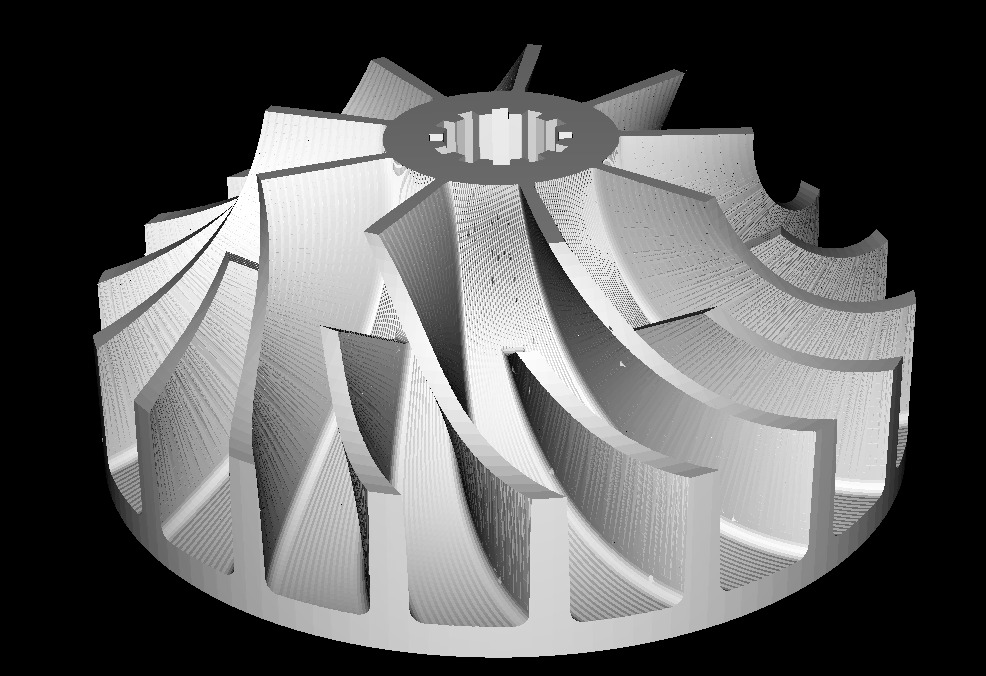
\includegraphics[width=0.49\textwidth]{multi_impeller}
\caption{Screenshot of the OpenCL kernel output of the SinglePrimaryBooleanCellRayCaster of a multi impeller.}
\label{fig:multi_impeller}
\end{figure}

\subsection{Development}

tools, debugger, VS integration

\subsection{Existing problems}

register consumption per work item (intersection buffer)

branch divergence

non coalesced memory access